\chapter [Discrete Fourier Transform]{Discrete Fourier Transform}


\section{AIM}
\begin{enumerate}
\item
Generate the sum of two sinewaves and analyse their spectrum.
\item
Find the DFT of given sequence and plot it.

\item
Find the circular convolution of two sequences.


\end{enumerate}
\section{THEORY}
\paragraph{}

Discrete fourier transform is found using the function fft(x,-1) and inverse discrete fourier transform using fft(x,1). To plot the magnitude and phase response, magnitude is found using the function abs(x) and phase using the function atan(imag(x),real(x)) .To find circular convolution of two signals x1(n) and x2(n) their corresponding dfts are found and multiplied to get Y(K)= X1(K)*X2(K).  IDFT of Y(K) gives y(n). To find circular convolution of two sequences both the sequences must be of same length and if not zeros are added to smallest sequence. 
\section{PROCEDURE}

\paragraph{}
\begin{enumerate}
\item
Start Scilab on PC and Scilab console window opens. Create a new blank SciNote.
\item
The code for the required program is typed and saved as Scilab SCE file with an extension .sci
\item

The continuous plots are made using the function $plot$ and discrete plots are made using the function $plot2d3$ with the corresponding $x$ axis and $y$ axis variables written inside paranthesis.

\item
To view all the plots in the same window the function $subplot$ is used.
\item
The results and the errors in the program are displayed in the console window.
The typed program is run using the $execute$.
\end{enumerate}

\section{SCILAB CODE}
\subsection{Frequency content of a sine wave}
\lstinputlisting[caption=Scilab code for finding frequency content in the sum of two sine waves]{./scilabCode/sine_dft.sci}



\subsection{DFT of a sequence}
\lstinputlisting[caption=Scilab code for finding frequency content in a sequence]{./scilabCode/dft_sequence.sci}


\subsection{Circular convolution using DFT}
\lstinputlisting[caption=Scilab code for finding circular confolution using dft]{./scilabCode/circular_conv.sci}


\section{RESULT}
Different signal operations were performed using SCILAB.
\begin{figure}
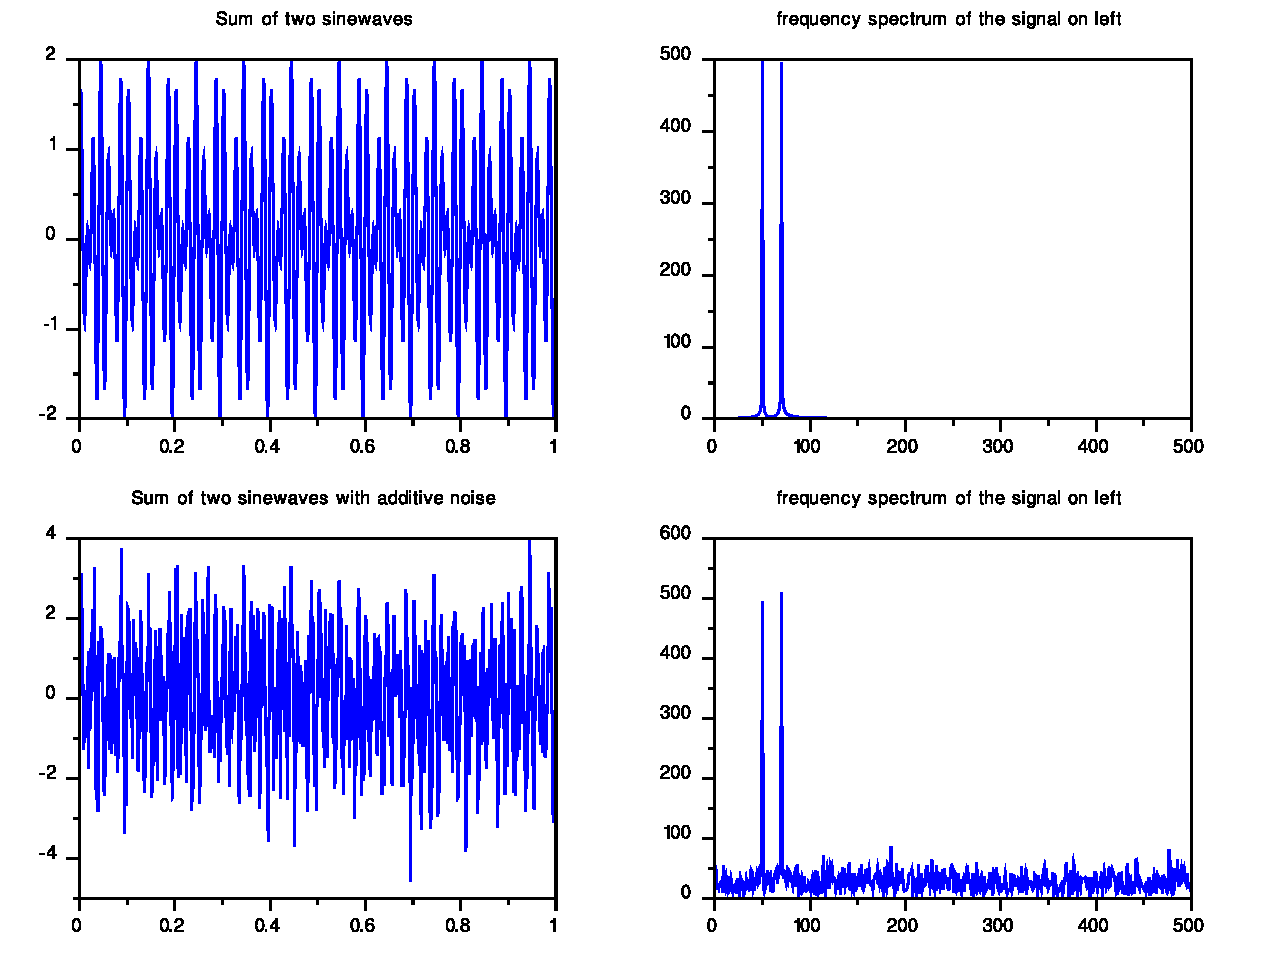
\includegraphics[scale=.5]{/home/kavya/kavyadev/DSPlab/scilabCode/sine_dft.pdf}
\caption{Plot of pure and noisy sine waves and their discrete Fouruer Transform}
\label{sine_dft}
\end{figure}

\begin{figure}
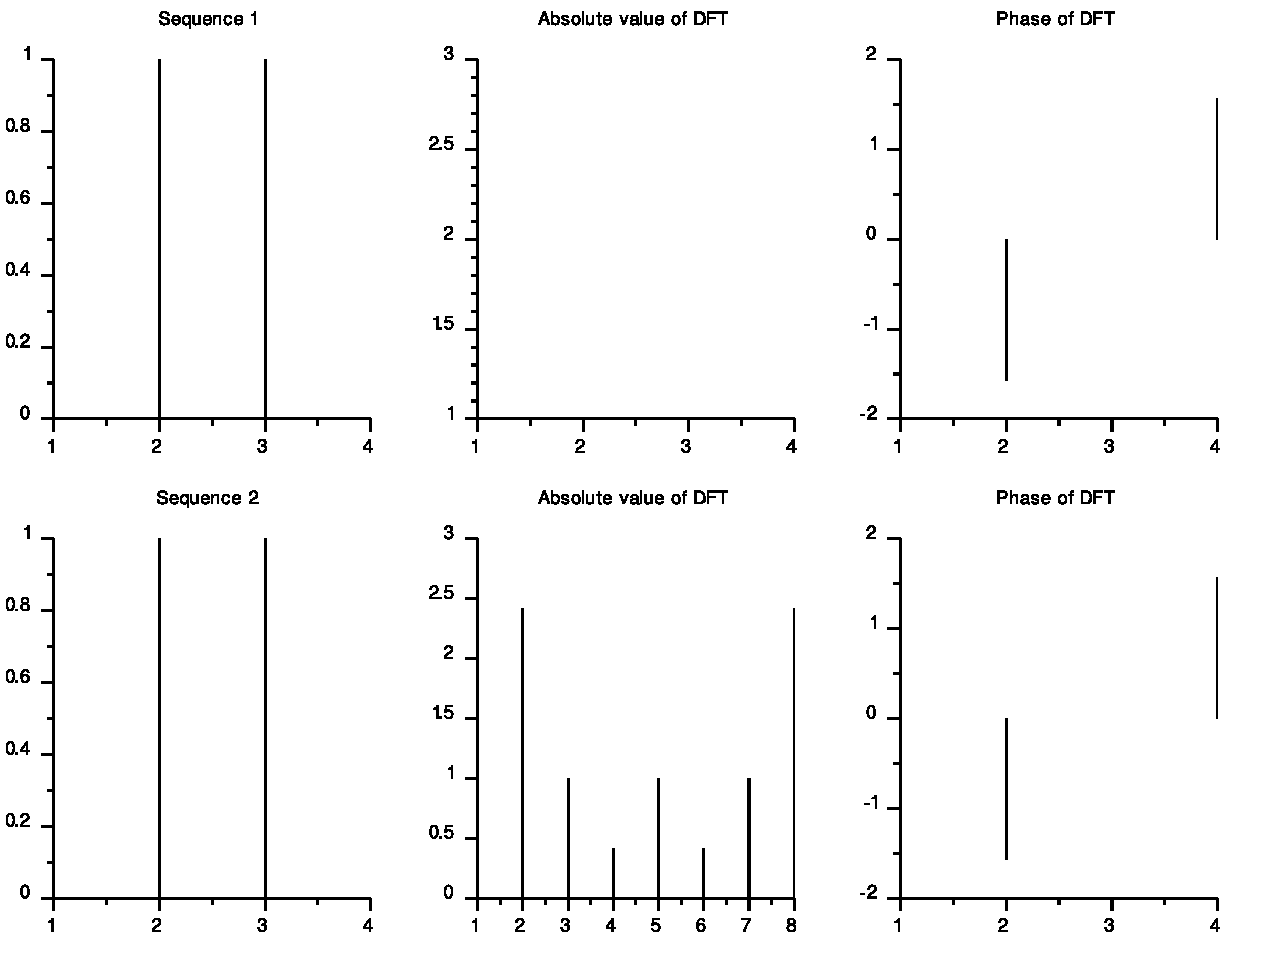
\includegraphics[scale=.5]{/home/kavya/kavyadev/DSPlab/scilabCode/dft_sequence.pdf}
\caption{Plot of a sequence and its DFT(magnitude and phase)}
\label{dft_sequence}
\end{figure}

\begin{figure}
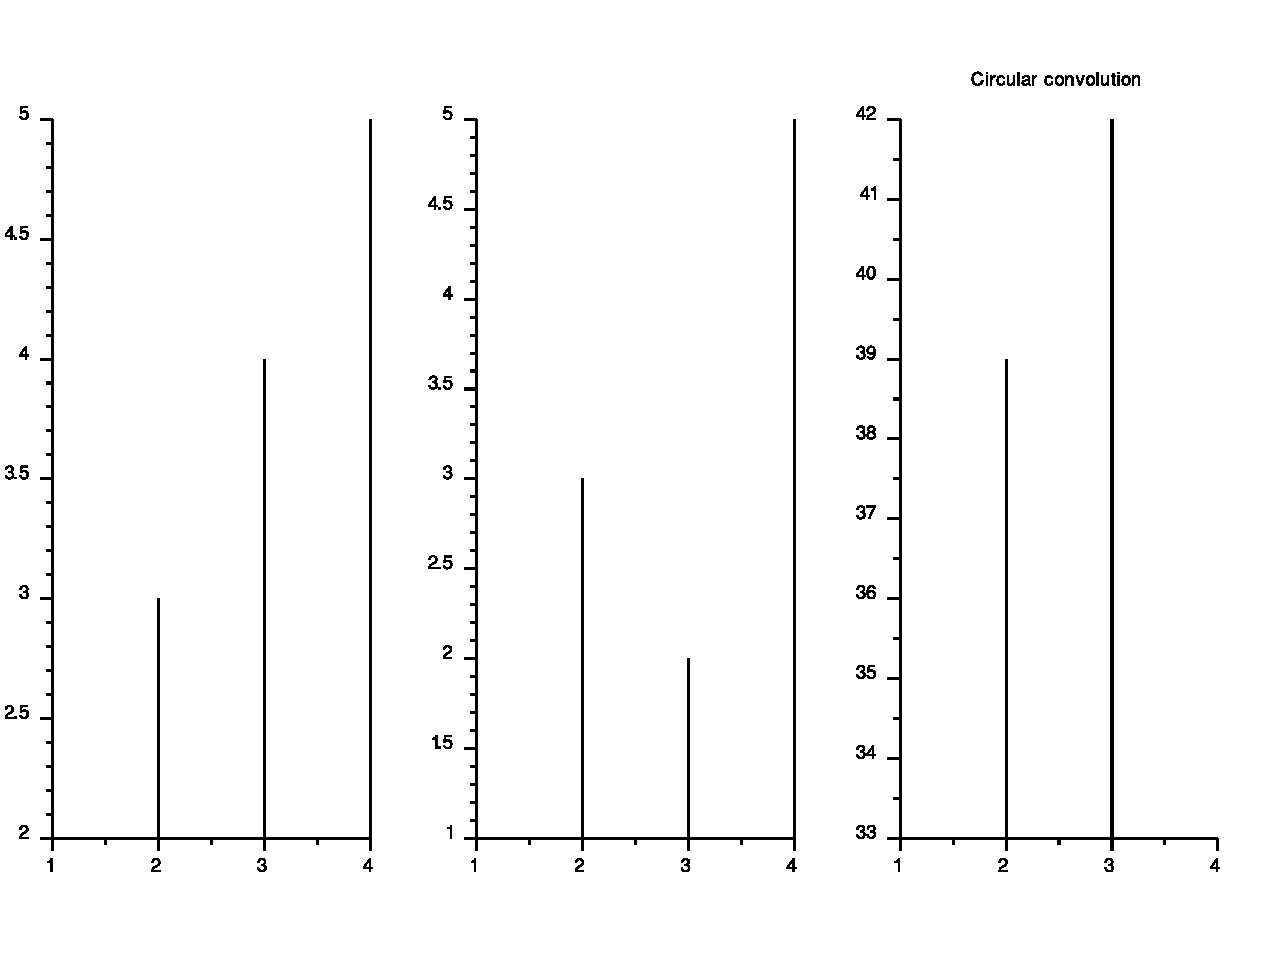
\includegraphics[scale=.5]{/home/kavya/kavyadev/DSPlab/scilabCode/circular_conv.pdf}
\caption{Plot of a sequence and its circular convolution}
\label{circular_conv}
\end{figure}